\section{Account Abstraction}
\label{sec:account_abstraction}

% Different solutions

Different solutions have been proposed to improve the user experience (UX) of web3.0 applications, including \textit{Meta Transactions}, \textit{Smart Contract Wallets}, and \textit{Account Abstraction}. The results of the analysis done by the Institute of Information Systems and Networking at the University of Applied Sciences and Arts of Southern Switzerland (SUPSI) indicate that \textit{Account Abstraction} presents the most promising solution for improving UX in decentralised systems, offering a comprehensive solution that enables smart contract logic to determine the fee payment and validation logic of transactions. \cite{isin-aa-user-experience}


%What is an account?
To analyse the concept of Account Abstraction, it is necessary to understand what an account is in the context of Ethereum, there are two types of accounts: \cite{ethereum-accounts}
\begin{itemize}
    \item \textit{Externally Owned Accounts (EOA)}: Controlled by anyone with the private key.
    \item \textit{Contract Accounts}: A deployed smart contract. Controlled by the code.
\end{itemize}

% Problem with EOA: fee, lost private key, etc.

EOAs are the only account type that can initiate transactions, while contract accounts can only \textit{react}\footnote{A smart contract can initiate a transaction by calling another smart contract, but the transaction is still initiated by an EOA.} to transactions. The main problem with EOAs is that they are not flexible enough to support the needs of modern applications. For example, EOAs can not be used to initiate batches of transactions and requires to always keep an ETH balance to cover gas. Other limitations include the lack of recovery options, the need to pay a fee for each transaction, and the risk of losing the private key. With these weaknesses, the user experience is not as seamless as in traditional web2.0 applications. \cite{ethereum-account-abstraction}

% What is account abstraction? Use a contract accounts instead of EOAs.
% Why use account abstraction? different use cases: recovery, relaying transactions, etc.

\textit{Account abstraction} is a way to solve these problems by allowing users to flexibly include more security and better user experiences into their accounts. This can happen in three ways: \cite{ethereum-account-abstraction}
\begin{itemize}
    \item \textit{Upgrading EOAs}: So that they can be controlled by Smart Contracts.
    \item \textit{Upgrading Smart Contracts}: So that they can initiate transactions. 
    \item \textit{Separate the transaction system}: Adding a second and separate transaction system.
\end{itemize}

The first two solutions require an upgrade of the Ethereum protocol, while the third solution can be implemented without changing the protocol.\cite{ethereum-account-abstraction} All possible paths will be discussed in the following sections.

Regardless of the route, the outcome is access to Ethereum via \textit{Smart Contract Wallets}, either natively supported as part of the existing protocol or via an add-on transaction network.  \cite{ethereum-account-abstraction}

The use of \textit{Smart Contract Wallets}  unlocks new possibilities, including: \cite{ethereum-account-abstraction}
\begin{itemize}
    \item \textit{Flexible security models}: Multi-signature, account freezing, transaction limits, allowlists, etc.
    \item \textit{Recovery options}: Social recovery, guardians, etc.
    \item \textit{Multi owner accounts}: Shared accounts, business accounts, etc.
    \item \textit{Relayed transactions}: Sign a transaction and let someone else pay for it.
    \item \textit{Batch/Multi transactions}: Execute multiple transactions in a single call.
    \item \textit{Innovative User Experience}: Seamless interaction with the blockchain.
\end{itemize}

% Write something to introduce EIP and Argent

In the following sections, the most relevant Ethereum Improvement Proposals (EIPs) related to Account Abstraction are presented. In particular, it is possible to notice how the community is advancing different solutions to achieve the same goal. Moreover, the Argent project is presented as an example of a real-world implementation of Account Abstraction.

\subsection{EIPs}
\label{subsec:eips}

The community of Ethereum is actively working to improve the blockchain. Everyone can propose an improvement through an EIP (Ethereum Improvement Proposal). An EIP is a design document providing information to the Ethereum community, or describing a new feature for Ethereum or its processes or environment. The EIP should provide a concise technical specification of the feature and a rationale for the feature. The EIP author is responsible for building consensus within the community and documenting dissenting opinions. \cite{eip-1}

In the context of Account Abstraction, the most relevant EIPs are in the category of \textit{Standards Track EIPs}, which are changes that affect most or all Ethereum implementations. Standards Track EIPs can also be classified into three categories: \cite{eip-1}
\begin{itemize}
    \item \textit{Core}: Changes that require a consensus (hard) fork.
    \item \textit{Networking}: Changes that affect network protocol, including changes that are specific to the network layer.
    \item \textit{Interface}: Includes improvements around language-level standards, like method names and contract ABIs.
    \item \textit{ERC}: Application-level standards and conventions, including contract standards such as token standards (ERC-20), name registries (ERC-137), URI schemes, library/package formats, and wallet formats.
\end{itemize}

\subsubsection{EIP-86}
\label{subsubsec:eip-86}

Proposed by Vitalik Buterin\footnote{co-founder of Ethereum} in 2017, EIP-86 is a \textit{Core} proposal and can be considered the first step towards account abstraction. The goal of this proposal is to abstract the signature verification and the nonce scheme. This allows to develop smart contracts able to use any signature scheme in transaction verification. \cite{eip-86}

The default way to secure an Ethereum account is the ECDSA\footnote{Elliptic Curve Digital Signature Algorithm \cite{ECDSA}} signature scheme. However, EIP-86 allows to use any signature scheme, including multi-signature schemes and \textbf{custom cryptography}. \cite{eip-86}

It is important to notice that ECDSA cryptography is \textbf{not} quantum-resistant, the Peter Shor's algorithm can be used to break the ECDSA in polynomial time. \cite{stewart2018committing}

The current status of EIP-86 is \textit{Stagnant}, as it has been inactive for more than 6 months. Nevertheless, this proposal was an inspiration for the following EIPs.

\subsubsection{EIP-2711} %Remove ???
\label{subsubsec:eip-2711}

Proposed in 2020, The EIP-2771 is based on the EIP-2718 proposal, which introduces a new transaction type. The main features that EIP-2771 may introduce are: \cite{eip-2711} 

\begin{itemize}
    \item \textit{Sponsored Transactions}: Allow third parties to pay for a user's gas costs.
    \item \textit{Batch Transactions}: Execute multiple transactions in a single call.
    \item \textit{Expiring Transactions}: Set an expiration time that invalidates the transaction.
\end{itemize}

To achieve these features, the concept of \textbf{meta-transaction} has been introduced. The idea is that transactions signed by a user get sent to a \textit{Forwarder} contract. The forwarder is a trusted \textbf{off-chain} entity that verifies that transactions are valid before sending them on to a gas relay. The forwarder passes the transaction on to a Recipient contract, paying the necessary gas to make the transaction executable on Ethereum. The transaction is executed if the Forwarder is known and trusted by the Recipient. This model makes it easy for developers to implement gasless transactions for users. \cite{ethereum-account-abstraction}

The proposal is a \textit{Core} EIP and it has been \textit{Withdrawn} by the author. The reason for the withdrawal is that the EIP-3074, proposed with the help of the EIP-2711 author, is a more complete solution. \cite{eip-2711}

\subsubsection{EIP-2938}
\label{subsubsec:eip-2938}

Proposed in 2020, The EIP-2938 is a \textit{Core} proposal that introduces a new EVM opcode\footnote{An Opcode is a machine-level instruction} called \texttt{PAYGAS}. As \hyperref[subsubsec:eip-2711]{EIP-2711}, also EIP-2938 is based on EIP-2718.

The main concept of EIP-2938 is to remove intermediaries during a relayed transaction. The implementations that need a Relayer are technically inefficient, due to the extra 21000 gas to pay for the relayer, economically inefficient, as relayers need to make a profit on top of the gas fees that they pay. Additionally, use of intermediary protocols means that these applications cannot simply rely on base Ethereum infrastructure and need to rely on extra protocols that have smaller userbases and higher risk of no longer being available at some future date. \cite{eip-2938}

Also the EIP-2938 is in a \textit{Stagnant} status, as it has been inactive for more than 6 months. The community is currently favouring EIP-4337. \cite{ethereum-account-abstraction}

\subsubsection{EIP-3074}
\label{subsubsec:eip-3074}

Proposed in 2020, EIP-3074 introduces two new opcodes to the Ethereum Virtual Machine (EVM): \texttt{AUTH} and \texttt{AUTHCALL}. The first sets a context variable authorized based on an ECDSA signature. The second sends a call as the authorized account. This essentially delegates control of the externally owned account (EOA) to a smart contract called \textit{Invoker}. The main purpose of EIP-3074 is to \textbf{upgrade EOAs}. \cite{eip-3074}

More specifically, \texttt{AUTH} enables the retrieval of a user's address from a signed message, effectively authenticating the user within EVM. \texttt{AUTHCALL}, on the other hand, simplifies the execution of authenticated calls by altering the sender of the transaction to the authorized address, thus simplifying the process of executing transactions that mimic smart contract logic directly from EOAs. \cite{ethereum-account-abstraction}

This gives developers a flexible framework for developing novel transaction schemes for EOAs. A motivating use case of this EIP is that it allows any EOA to act like a smart contract wallet without deploying a contract (many EOAs may use the same \textit{Invoker} contract). \cite{eip-3074}

The \textit{Invoker} contract is a trustless intermediary between the EOA and the rest of the Ethereum network. The contract can be used to implement a variety of features, such as \textit{sponsored transactions}, \textit{expiration}, \textit{batch transactions}, etc. \cite{eip-3074}

As stated in the EIP: \cite{eip-3074}
\begin{displayquote}
    Choosing an invoker is similar to choosing a smart contract wallet implementation. It's important to choose one that has been thoroughly reviewed, tested, and accepted by the community as secure. We expect a few invoker designs to be utilized by most major transaction relay providers, with a few outliers that offer more novel mechanisms.
\end{displayquote}

EIP-3074 is currently in \textit{Review} status, and it is expected to be included in the next hard fork of Ethereum, named \textit{Pectra}, expected in Q4 2024. \cite{pectra-hardfork}

\subsubsection{ERC-4337}
\label{subsubsec:erc-4337}

Proposed in 2021, ERC-4337 is an account abstraction proposal which completely avoids the need for consensus-layer protocol changes by creating a \textbf{separate transaction system}. \cite{eip-4337}

Instead of adding new protocol features and changing the bottom-layer transaction type, this proposal introduces a higher-layer pseudo-transaction object called a \textit{UserOperation}. 
As illustrated by figure \ref{fig:4337-diagram}, users send \textit{UserOperation} objects into a separate \textit{mempool}. A special class of actor called bundlers package up a set of these objects into a transaction making a \textit{handleOps} call to a special contract, and that transaction then gets included in a block. 

\begin{figure}[H]
    \centering
    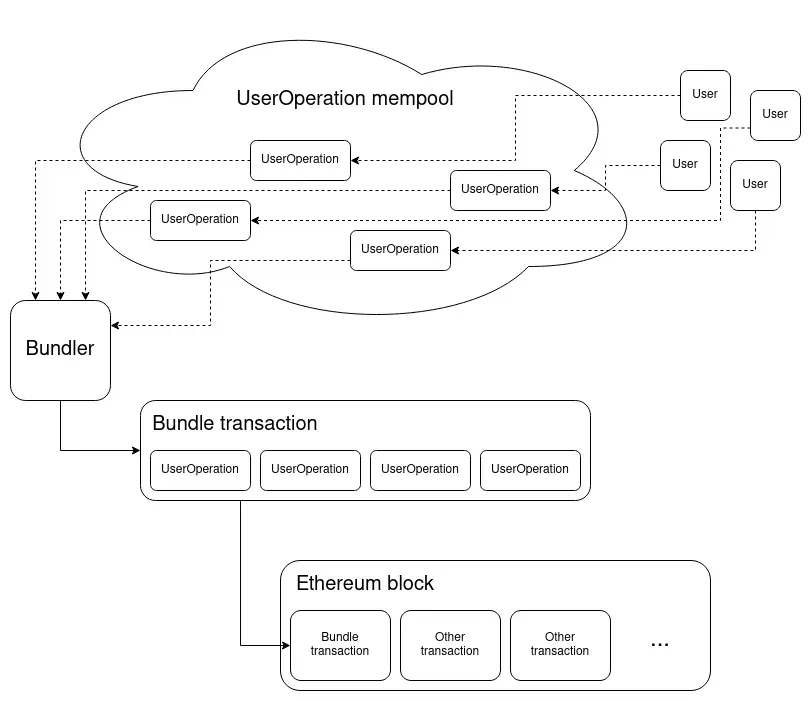
\includegraphics[width=0.8\linewidth]{state_of_the_art/4337-diagram}
    \caption{ERC-4337 Diagram}
    \label{fig:4337-diagram}
\end{figure}


ERC-4337 also introduces a paymaster mechanism that can enable users to pay gas fees using ERC-20 tokens (e.g. USDC) instead of ETH or to allow a third party to sponsor their gas fees altogether, all in a decentralized fashion. \cite{isin-aa-user-experience}

The ERC-4337 is in \textit{Draft} status and the main start contract required was deployed in March 2023. \cite{ethereum-roadmap-ux}

\subsubsection{EIP-7702}

Proposed in 2024 co-authored by Vitalik Buterin, EIP-7702 is the latest proposal for account abstraction. The main goal of this proposal is to offer the same features as \hyperref[subsubsec:eip-3074]{EIP-3074}, but without the need of the two opcodes \texttt{AUTH} and \texttt{AUTHCALL}. The reason is that, as stated in the EIP, the two opcodes will not be used in the final solution for Account Abstraction, where Smart Contract Wallets will eventually be implemented. \cite{eip-7702}

EIP-7702 propose to a new transaction type that adds a \texttt{contract\_code} field and signature, the idea is to convert the signing account (not necessarily the same that started the transaction) into a smart contract wallet for the duration of that transaction. \cite{eip-7702}

This \textit{Core} proposal is in an early stage, as it is in \textit{Draft} status. But it is promising, as it is co-authored by Vitalik Buterin, one of the co-founders of Ethereum.

\subsection{Argent}
\label{subsec:argent}

Argent\footnote{https://www.argent.xyz/} is a well known company whose mission is to make blockchain widely used. To achieve this goal, Argent, as a pioneer in the field of Account Abstraction, has developed different solutions to improve the user experience of blockchain applications. \cite{argent-aa}

One of the first solutions developed by Argent is the open source project \textit{Argent Wallet Smart Contract}. The Argent wallet is an Ethereum Smart Contract based mobile wallet. The wallet's user keeps an EOA secretly on his mobile device. This account is set as the owner of the Smart Contract. User's funds (ETH and ERC20 tokens) are stored on the Smart Contract. With that model, logic can be added to the wallet to improve both the user experience and the wallet security. \cite{argent-github}

% Argent does not use the EIPs, because they are not yet implemented in the Ethereum mainnet. but with a more complex solution, they have achieved the same goal.

Argent smart contracts do not use the \hyperref[subsec:eips]{EIPs} presented in the previous section, as the major of them need a hard fork to be implemented in the Ethereum Mainnet. Instead, Argent has developed a more complex solution to achieve the same goal. 

% Argent functionalities

The functionalities of the Argent wallet are: \cite{argent-smart-wallet-specifications}
\begin{itemize}
    \item \textit{Guardians}: Authorized accounts (EOA or smart contracts) permitted by the wallet owner to execute specific operations such as locking, unlocking, initiating recovery procedures, approving transactions to unknown accounts, or creating session keys. Guardians can be various entities including friends' wallets, EOAs, hardware wallets, or paid third-party services. Adding or removing guardians requires confirmation within a specified time frame to prevent unauthorized access.
    \item \textit{Recovery}: Mechanism allowing wallet owners to regain access to their funds in case of loss or compromise, typically involving a predefined recovery process facilitated by designated guardians. Recovery processes require validation by the wallet's guardians and can be cancelled or finalized within a certain time frame.
    \item \textit{Ownership Transfer}: Allows users to transfer ownership of their wallet to a new device while still in possession of the original device. The transfer is immediate to avoid service interruption but requires approval from guardians.
    \item \textit{Multi-Call}: Enables the wallet to interact with the Ethereum ecosystem by executing a sequence of transactions one after the other. The multi-call fails if any of the transactions fail and requires specific conditions to be met for execution.
    \item \textit{Trusted Contacts}: Allows users to maintain a list of trusted addresses managed by the wallet owner. Interacting with trusted contacts, such as sending assets, does not require additional authorization.
    \item \textit{Dapp Registry}: Supports two registries of authorized addresses, including native integration dapps and curated dapps accessible through WalletConnect. Entries in the registry are time-locked and require guardian approvals for enabling or disabling.
    \item \textit{Session}: Users can execute multiple transactions within a given time window with guardian approval, required only once by creating a session with a temporary session key.
    \item \textit{Upgradability}: Allows for the wallet to be upgraded to add new features or fix potential bugs, with the choice left to the wallet owner without the ability for a centralized party to force an upgrade.
    \item \textit{ETH-Less Account}: Enables owner and guardians to execute wallet operations without owning ETH or paying transaction fees by utilizing \textit{Meta Transactions}, where a third-party relayer executes transactions on their behalf.
    \end{itemize}
    
\subsubsection{Argent Wallet Smart Contract Architecture}

The simplified architecture of the Argent Wallet Smart Contract is shown in attachment \embedfileandcreatelink{attachments/A1-ArgentWalletsOriginal.png}{\textit{A1-ArgentWalletsOriginal}}, where the main components are: \cite{argent-smart-wallet-specifications}

\begin{itemize}
    \item \textit{Wallet Factory}: Wallet factory contract used to create proxy wallets using \texttt{CREATE2}\footnote{Gives the ability predict the address where a contract will be deployed, without ever having to do so. \cite{opcode-create2}} opcode and assign them to users.
    \item \textit{Base Wallet and Proxy}: The Base Wallet is a simple library-like contract implementing basic wallet functionalities that are not expected to ever change. These functionalities include changing the owner of the wallet, (de)authorizating modules and performing (value-carrying) internal transactions to third-party contracts. The Proxy Wallet is a contract that delegates all calls to the Base Wallet, the goal is to reduce the deployment cost of each new wallet.
    \item \textit{Module Registry}: The Module Registry maintains a list of the registered Module contracts that can be used with user wallets.
    \item \textit{Argent Module}: All the functionalities of the Argent wallet are currently implemented in a single module. To structure the code, the \textit{ArgentModule} inherits from several abstract managers that each implements a coherent subset of the logic:
        \begin{itemize}
            \item \textit{Transaction Manager}: Manages the execution of multi-calls, adding or removing trusted contacts and session executions.
            \item \textit{Security Manager}: Manages the wallet's security features, including guardians, recovery, locking and ownership transfer.
            \item \textit{Relayer Manager}: Entry point for Meta Transactions, allowing users to execute transactions without owning ETH.
        \end{itemize}
    \item \textit{Dapp Registry}: The Dapp Registry is a contract that maintains a list of dapps that are allowed to interact with the wallet.
    \item \textit{Storages}: The wallet's state is stored in two separate storage contracts:
    \begin{itemize}
        \item \textit{Transfer Storage}: Used to store the trusted contacts of a wallet.
        \item \textit{Guardian Storage}: Used to store the list of guardians of a wallet.
    \end{itemize}
\end{itemize}